\chapter{Related Work} \label{ch:related_work}

In this chapter, we will give an overview of related work that examines, similar to ours, the performance of different NLDR methods. Most of the related work introduced in the following is partially related to this work because not all methods that our work will compare are addressed in the related work. This work compares the NLDR methods of nonlinear MDS, LLE, and t-SNE.

\section{Speed and Accuracy Evaluations} \label{sec:speed_and_accuracy}

Although we will not compare the DR methods' runtime performances, some articles address this. We still want to introduce an exemplary one from Zubova et al. \cite{Zubova18}, where they also compared the accuracy of the methods with a focus on big data.

The two criteria they used for their comparisons were, on the one hand, the speed meaning the execution time of the method, and on the other hand, the accuracy using three different measures that we will not further elaborate on. The datasets they used were categorized into three groups, but we will summarize two into one because they showed no different behaviors and results. The first group of datasets was randomly generated, and the data for the second group was extracted from a real-world financial scenario.

The results of the researchers' experiments were that for the randomly generated data, the increase of instances had an impact on the execution time but no impact on the accuracy of the methods. Whereas the increase of initial dimensions impacted the criteria the other way around, meaning that the execution time was not affected, but the accuracy was worse. Also, as expected, the nonlinear methods were much slower than the linear methods because nonlinear methods search for more complex structures in the data. Furthermore, MDS was the most accurate of all compared methods, and LLE was the least accurate. Overall, regarding the generated data, LLE is slightly faster than MDS but much less accurate than the latter.

The behaviors of the DR methods that were compared concerning the impact of the increase of dimensions and instances were similar to the investigations with the randomly generated data. But there was an exception that increased instances led to higher accuracy. The researcher also identified the anomaly that the execution time of MDS was increased with dimensions that can be considered unusual when looking at previous results. The reasons for this are unknown to the researchers; therefore, further research must be conducted. In this real-world example, the researchers could also not generate results for the LLE method because it did not finish its execution on those datasets. This further proves that real-world data is much more complex and can't be easily mimicked by synthetic data.

\section{Visualization Evaluations} \label{sec:vis_eval}

In the work of Akhbardeh and Jacobs \cite{Akhbardeh12}, linear and nonlinear DR techniques were compared with each other in terms of how well they can preserve the structure of high dimensional data and under the aspect of visualization. The two types of high dimensional data they used for comparison tasks were, on the one hand, synthetic data such as the famous Swiss roll \ref{fig:swiss_roll_related_work}, 3-clusters \ref{fig:3-cluster_related_work}, and a sparse nonuniform manifold \ref{fig:sparse_related_work}, and on the other hand, real breast magnetic resonance imaging (MRI) that were pre-processed beforehand and then applied on several DR methods. 

All synthetic examples were embedded from a 3-dimensional space into a two-dimensional space. Classic MDS, LLE, and other techniques, such as ISOMAP and Diffusion maps, were used for all comparisons. Those other techniques aren't relevant to this work and will not be mentioned further. Important to note: for LLE, the neighborhood size was across all investigations set to 5. The researchers found out that for the synthetic data investigations, the LLE technique resulted in a mostly successful reduction of the dimensions of the manifolds. In contrast, classic MDS mostly failed to preserve the structure. Overall, LLE outperformed classic MDS regarding synthetic data investigations.

In particular, classic MDS failed to unfold the Swiss roll, but LLE was able to unfold and preserve the structure of the manifold partly, as shown in Fig. \ref{fig:swiss_roll_related_work}.
\begin{figure}[!]
	\centering
	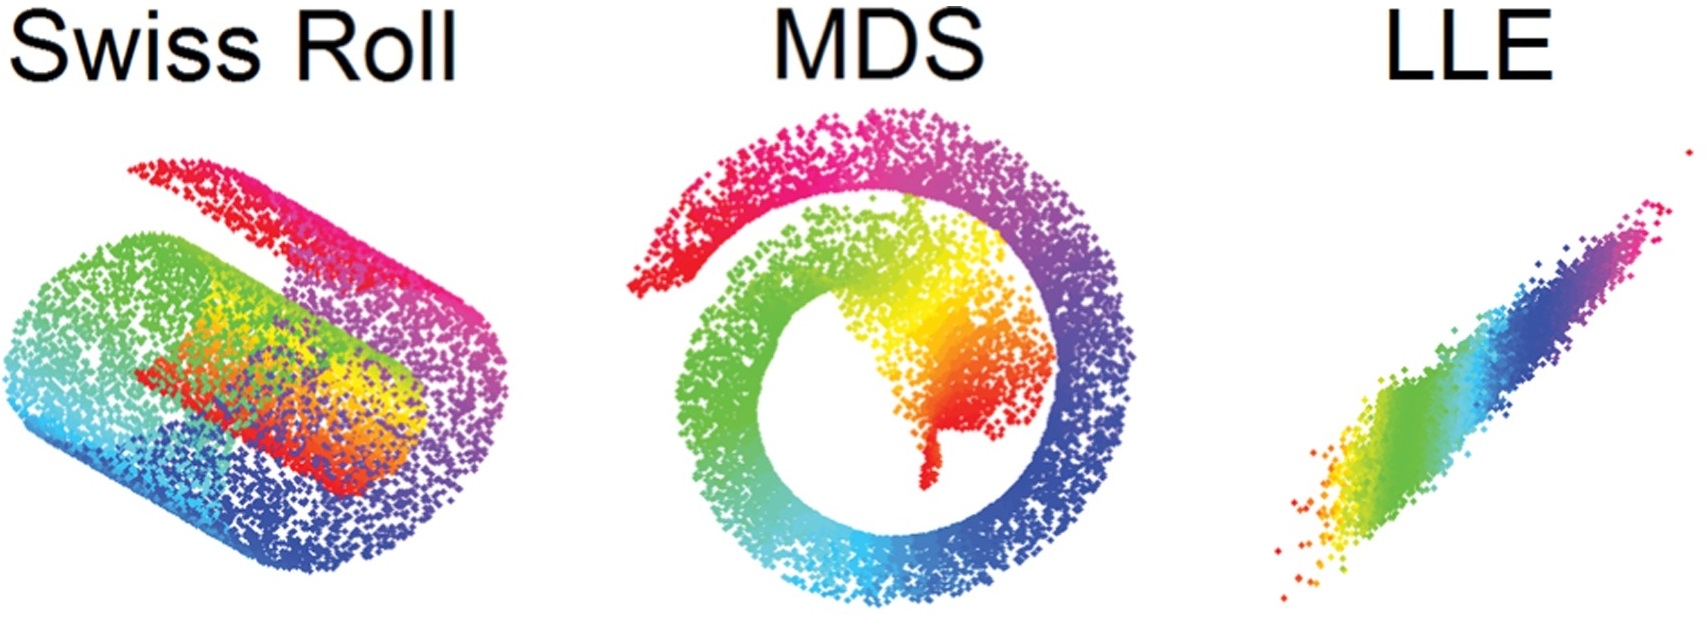
\includegraphics[width=\columnwidth-0.4cm]{images/swiss_roll_related_work.jpg}
	\caption[Dimensionality Reduction on Swiss Roll]{Dimensionality Reduction on Swiss Roll adapted from Fig. 5 in \cite{Akhbardeh12}}
    \label{fig:swiss_roll_related_work}
\end{figure}
For the 3-cluster example, all used methods, but LLE yielded good results. The clusters collapsed into points, not modifying the clusters but the overall structure, as shown in Fig. \ref{fig:3-cluster_related_work}.
\begin{figure}[!]
	\centering
	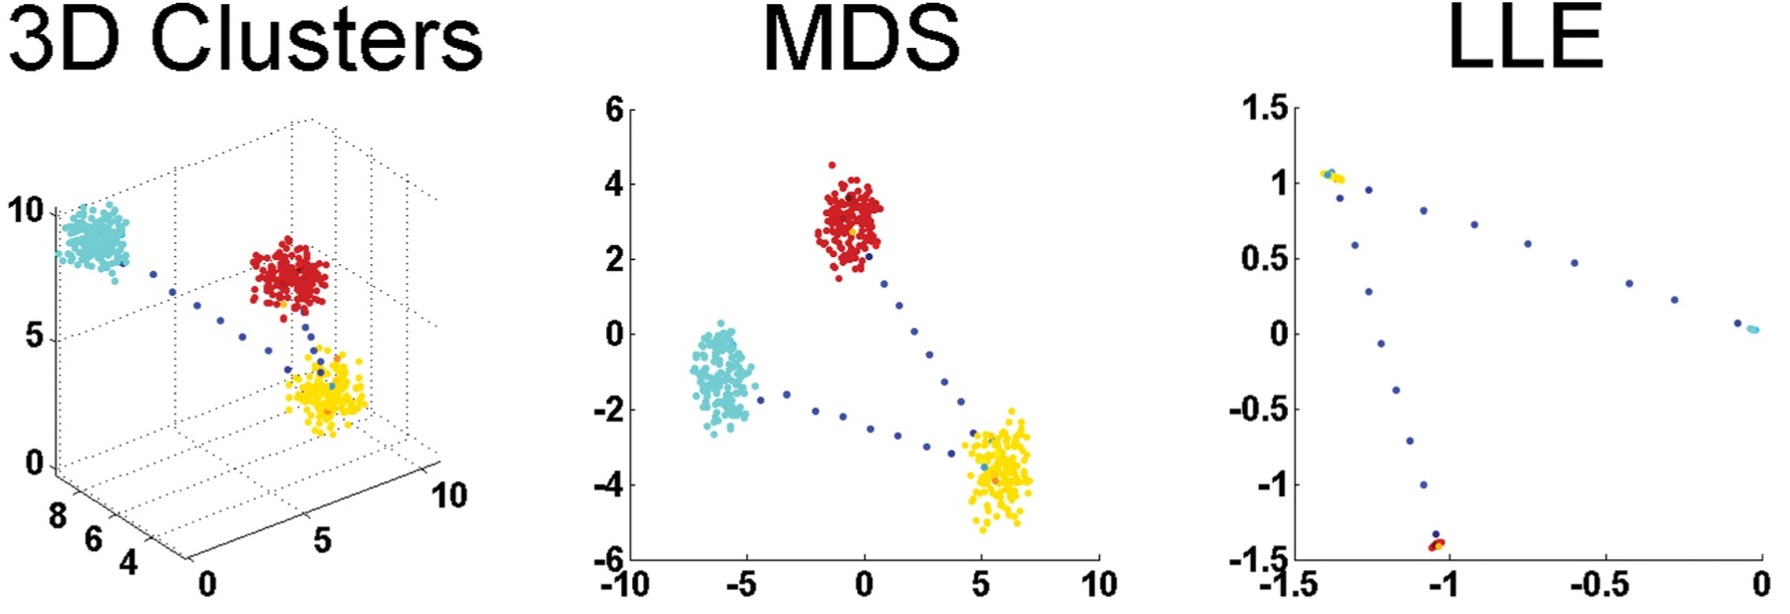
\includegraphics[width=\columnwidth-0.4cm]{images/3-cluster_related_work.jpg}
	\caption[Dimensionality Reduction on 3-Clusters]{Dimensionality Reduction on 3-Clusters adapted from Fig. 6 in \cite{Akhbardeh12}}
    \label{fig:3-cluster_related_work}
\end{figure}
The sparse nonuniform manifold example was a more complex dataset. As the researchers expected, the linear methods, such as classic MDS, failed to preserve the structure, whereas the nonlinear methods, such as LLE, performed well, as shown in Fig. \ref{fig:sparse_related_work}.
\begin{figure}[!]
	\centering
	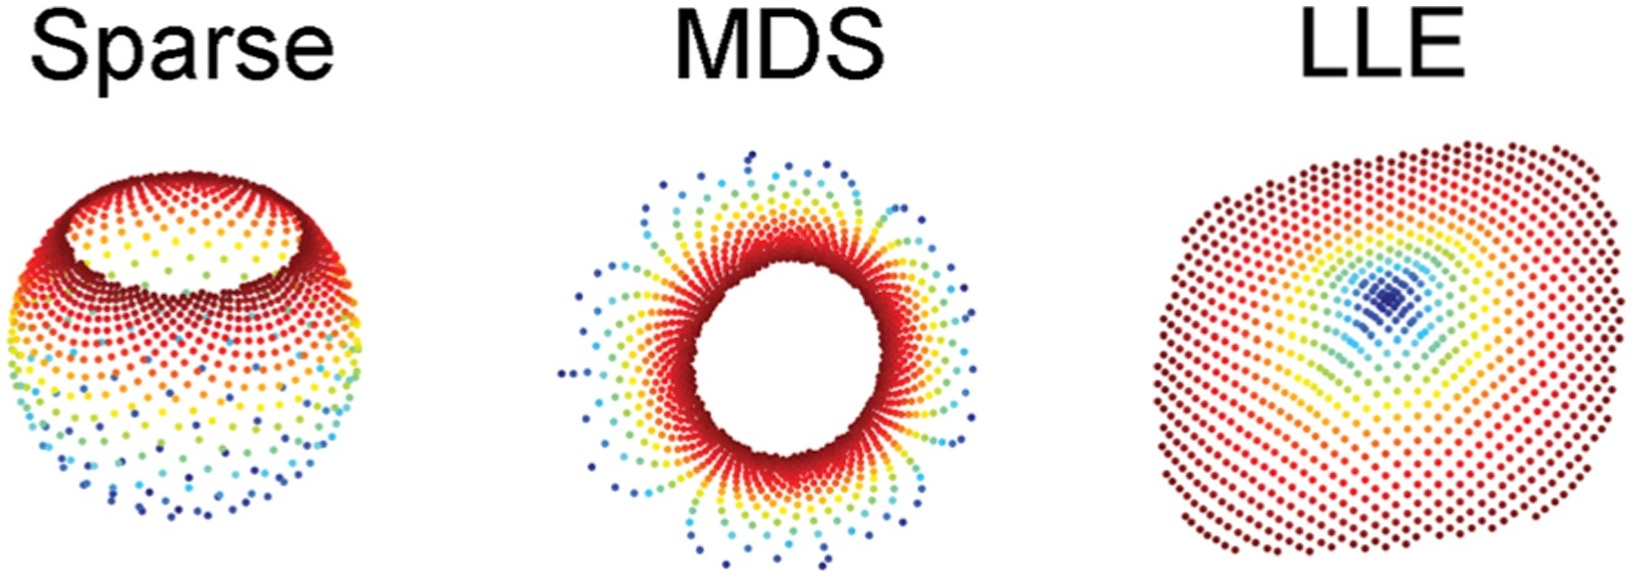
\includegraphics[width=\columnwidth-0.4cm]{images/sparse_related_work.jpg}
	\caption[Dimensionality Reduction on Sparse Nonuniform Manifold]{Dimensionality Reduction on Sparse Nonuniform Manifold adapted from Fig. 7 in \cite{Akhbardeh12}}
    \label{fig:sparse_related_work}
\end{figure}

The task on the images of the real clinical data was to visualize radiological data and segment normal from abnormal tissues. The MRI parameters were considered as the dimensions of the original space, and the task was to embed it into a single image. In this task, just the nonlinear DR methods were used. The result of the works was that the NLDR methods segmented different breast tissue types and successfully visualized the various tissues and their boundaries with high accuracy. Furthermore, they investigated the methods concerning the robustness of their input parameters. In LLE, the input parameter is the neighborhood size K, with inputs ranging from 0 to 200. The result was that LLE was most robust when choosing K in the 20 to 60 range, as shown in Fig. \ref{fig:LLE_robustness_related_work}.
\begin{figure}[!]
	\centering
	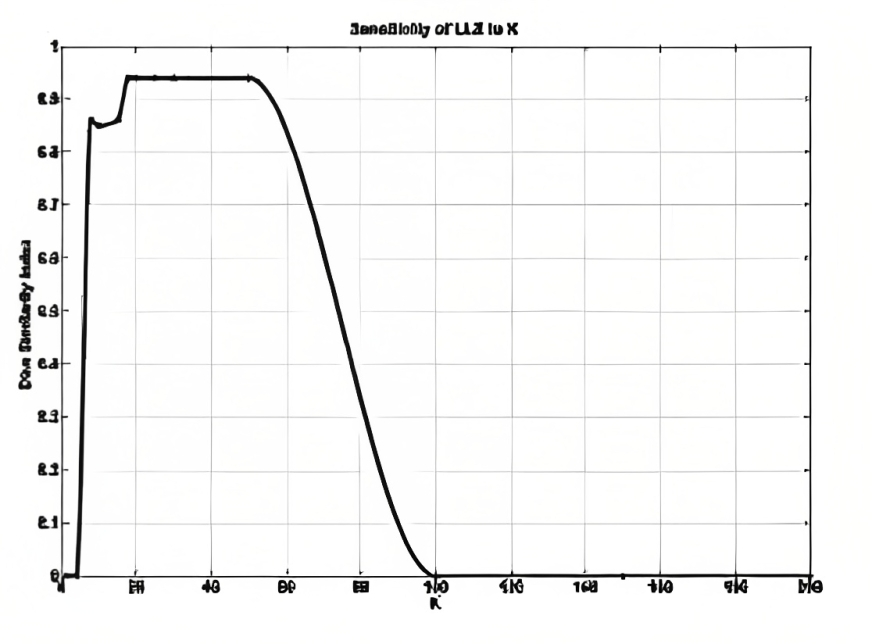
\includegraphics[width=\columnwidth]{images/LLE_robustness_related_work.jpg}
	\caption[Sensitivity to input parameter choice for LLE]{Sensitivity to input parameter choice K for LLE adapted from Fig. 13 in \cite{Akhbardeh12}}
    \label{fig:LLE_robustness_related_work}
\end{figure}

The researchers found out that all of the nonlinear DR methods they compared were suitable for this specific task of processing MRI data to analyze the different tissue types. Moreover, they found out that LLE has the advantage over other methods in that it can preserve the local structure well but therefore has less sensitivity to the variation in the global structure in datasets.

\section{Cluster Evaluations} \label{sec:clu_eval}

In the work from Vasighizaker et al., \cite{Vasighizaker22}, they investigated how applying dimensionality reduction first affects the performance of clustering on single-cell RNA-Sequences (scRNA-seq) to identify their belonging to specific cell types. Before the use of DR was considered in this field, the usage of clustering algorithms alone was state-of-the-art, but using them alone has a significant drawback. Most of the time, scRNA-seq data has high dimensionality that is also sparse. This results in computationally intensive applications of clustering algorithms. This is why applying dimensionality reduction first was considered a good practice.

To compare different DR methods, they used 13 publicly available scRNA-seq datasets of different tissues, sizes, and technologies that the researchers pre-processed to ensure high data quality. Those datasets were then reduced to 3 dimensions by applying the following DR methods: ISOMAP, Laplacian Eigenmap, PCA, t-SNE, LLE, and modified LLE. In this work, we will just consider the nonlinear DR methods t-SNE and LLE because the other ones are not in the scope of this work. After that, the clusters were formed by applying k-means. The best combination of parameters to choose for the different methods was discovered by applying a grid search and comparing the silhouette score of the results. Important to note that statistical and biological tools were used to generate the ground truth clustering. The higher the silhouette score, the better the overall cluster quality is, ranging from 0 to 1. Based on all 13 datasets, t-SNE had an average silhouette score of 0.248 (Standard deviation: 0.034) and LLE of 0.570 (Standard deviation: 0.113). 

Now we want to give a closer look into one specific dataset, namely H1299 scRNA-seq. The silhouette score for this dataset for t-SNE was 0.245 and for LLE, 0.683. Fig. \ref{fig:3d_related_work} shows the reduced and clustered dataset.
\begin{figure}[!]
	\centering
	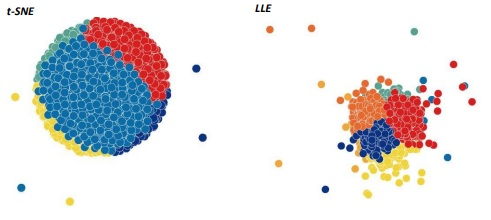
\includegraphics[width=\columnwidth]{images/3d_related_work.jpg}
	\caption[Dimensionality reduction and k-means clustering]{Dimensionality reduction into 3 dimensions of H1299 scRNA-seq dataset with k-means clustering adapted from Fig. S5 in \cite{Vasighizaker22}}
    \label{fig:3d_related_work}
\end{figure}
To further reduce the dimension from 3D to 2D, the linear DR method of Independent component analysis (ICA) was employed. The authors claim this has the advantage of enhancing the visualization of clustered 3-dimensional data. This claim is founded on their observation of "well-marked 'lines' or 'axes'". They also say that "applying ICA reveals some hidden, complex relationships among the cells in the clusters, which are not noticeable in three dimensions." \cite{Vasighizaker22} After this second dimensionality reduction on the dataset, k-means has to be performed again. In Fig. \ref{fig:t-sne_related_work}, one can see the results of the t-SNE method. In Fig. \ref{fig:lle_related_work}, one can see the results of the LLE method.
\begin{figure}[!]
	\centering
	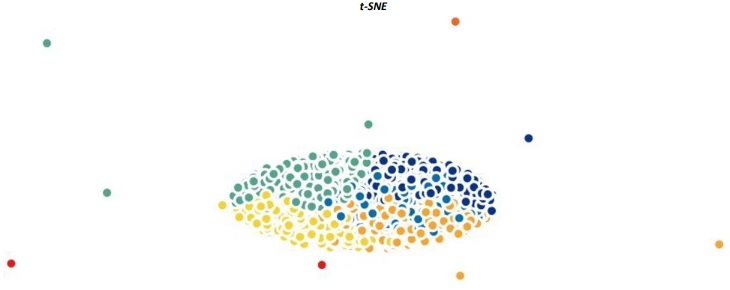
\includegraphics[width=\columnwidth]{images/t-sne_related_work.jpg}
	\caption[t-SNE dimensionality reduction and k-means clustering]{t-SNE dimensionality reduction into 3 dimensions and ICA dimensionality reduction into 2 dimensions of H1299 scRNA-seq dataset with k-means clustering adapted from Fig. 5 in \cite{Vasighizaker22}}
    \label{fig:t-sne_related_work}
\end{figure}
\begin{figure}[!]
	\centering
	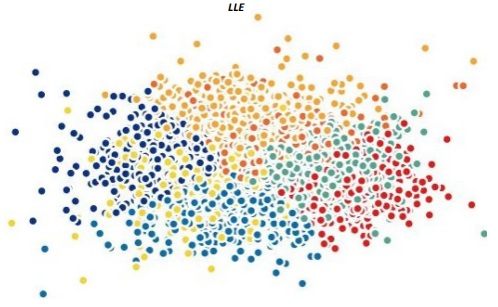
\includegraphics[width=\columnwidth]{images/lle_related_work.jpg}
	\caption[LLE dimensionality reduction and k-means clustering]{LLE dimensionality reduction into 3 dimensions and ICA dimensionality reduction into 2 dimensions of H1299 scRNA-seq dataset with k-means clustering adapted from Fig. 9 in \cite{Vasighizaker22}}
    \label{fig:lle_related_work}
\end{figure}

Although the modified LLE method is not in the scope of this work, it is important to note that the best results regarding the silhouette score were achieved by this method with post-ICA application. Modified LLE itself had similarly good results. It stands out that t-SNE has very bad and LLE has moderate results. The researchers point out that this outcome might depend on using k-Means as a clustering algorithm. Other algorithms, such as DBSCAN, might have generated better clustering results.

\section{What it means for us} \label{sec:what_does_this_mean_for_us?}

We have looked over some articles that focused on comparing different DR methods. From those, we have extracted the knowledge that nonlinear DR methods mostly outperform linear DR methods. \ref{sec:vis_eval} That is due to the fact that the world consists of and generates complex and high-dimensional data that most likely does not contain linear structures. We also extracted the fact that some DR methods probably need specific clustering algorithms that can exploit the learned lower-dimensional representations from the DR methods and therefore lead to a better clustering result. For example, we have seen that t-SNE, in combination with k-Means, performed poorly. \ref{sec:clu_eval}

The current research on the topic of comparing DR methods shows us that it is needed to conduct more research of this type, since (a) the literature landscape of comparing such DR methods is relatively sparse and (b) there is a need to investigate and highlight the capabilities and boundaries of DR methods for the scientific community. One of the major problems of the current research is that it is domain-specific and therefore does not convey the opportunities to make general statements or recommendations. Our work aims to overcome this issue by comparing different methods on different domains and synthetic data designed to represent the real world as accurately as possible. On those datasets, we will investigate the behaviors of the DR methods and analyze why and in what context they behave a certain way. For this purpose, we will use some of the suggested quantitative evaluation measures discussed in the article from Gisbrecht et al. \cite{Gisbrecht15}. We will further elaborate on this in Chapter \ref{cap:methodology}.

But before diving into the experiments, it is however deemed necessary to establish a profound understanding for the reader of the theoretical foundation of the manifold task itself and the different manifold learning methods.